\documentclass{article}
\usepackage[utf8]{inputenc}
\usepackage{graphicx}
\usepackage{subcaption}
\usepackage[bottom=0.5in,top=0.5in,right=1in,left=1in]{geometry}
\usepackage[section]{placeins}
\usepackage{float}
\title{Experiment 4}
\author{Nitish Kumar Thakur \\ 21531010 }
\date{24 August, 2021}

\begin{document}

\maketitle

\section{Objective}
1.Obtain and plot the VCO characteristics of IC-8038 \par
2.Design and fabricate an FM modulator using IC-8038
 
 \section{Components and Equipment Required}                    
 IC-8038 *DSO *Power supply (variable)*connecting wire *Breadboard *probes *Resistance *DSO *Function generator
 
\section{Theory}

\subsection{FM Modulation}
In Frequency Modulation technique, Message signal voltage variation will be converted corresponding carrier signal frequency variation.this is known as Frequency modulation.\par
if we observe the below figure there is Three waveform first one is Message signal second one carrier signal and 3rd one is a Modulated signal.when amplitude of message signal is positive peak we see waveform is closely in time domain that means frequency is high and when message signal attend negative peak we see frequency is very low.that means information associated in Frequency Modulation technique in the form of carrier signal frequency variation.

\begin{figure*}[h]
	\centering
	\includegraphics[scale=0.65]{23.png}
	\caption{FM Modulation}
	\label{FBD}
\end{figure*}


\subsection{Voltage Controlled Oscillator}
Voltage-controlled oscillator is electronic oscillator the work of VCO is when we give variable voltage in VCO it generates varying frequency curve(Linear).This thing shown in below Figure
In this experiment VCO circuit achieved by IC-8038

\begin{figure*}[h]
	\centering
	\includegraphics[scale=0.6]{22.png}
	\caption{Voltage-controlled oscillator}
	\label{FBD}
\end{figure*}




\subsubsection{IC-8038}
IC-8038 is 14 pin ic,which is used to generate  high accuracy sine, square,triangular, sawtooth and pulse waveforms.\par

\begin{figure}[ht]
  \begin{subfigure}[b]{0.5\textwidth}
    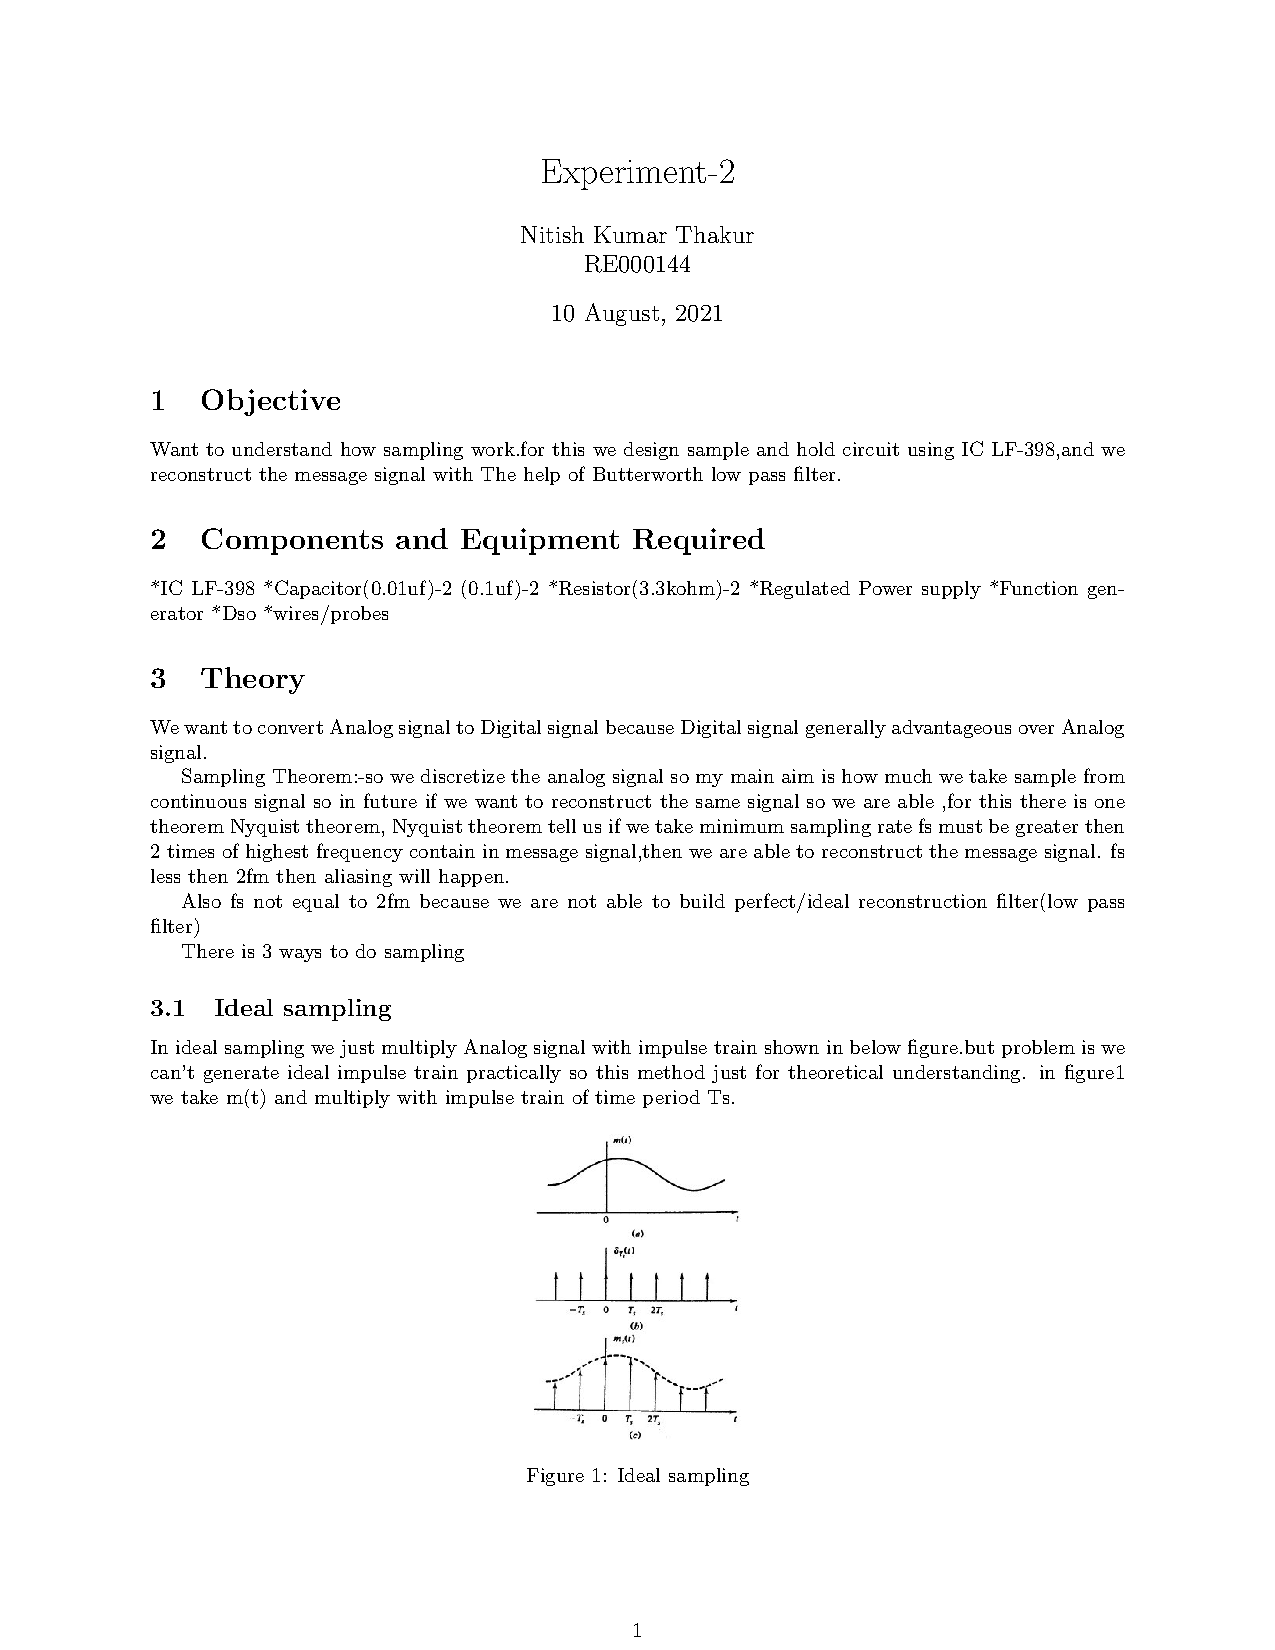
\includegraphics[width=\textwidth]{2.png}
    \caption{Top view of IC-8038}
    \label{fig:1}
  \end{subfigure}
  %
  \begin{subfigure}[b]{0.5\textwidth}
    \includegraphics[width=\textwidth]{1.1.png}
    \caption{Functional Diagram of IC-8038}
    \label{fig:2}
  \end{subfigure}
\end{figure}

\subsection{Frequency Modulation and Sweeping}
Frequency at output of IC is direct function of DC voltage at pin-8.For small deviations (e.g. ±10\% ) the modulating signal can be applied directly to pin 8.an external Resistor between pin7-8 is not necessary\par
For larger FM deviations or for frequency sweeping, the message signal is applied between supply voltage and pin 8.In this way the entire bias for the current sources is created by the Message signal, and a very large  sweep range is created.in this configuration(Fig(b)) the charge current is no longer a function of the supply voltage and the frequency becomes dependent on the supply voltage.
\begin{figure}[ht]
  \begin{subfigure}[b]{0.4\textwidth}
    \includegraphics[width=\textwidth]{20.png}
    \caption{CONNECTIONS FOR FREQUENCY MODULATION}
    \label{fig:1}
  \end{subfigure}
  %
  \begin{subfigure}[b]{0.4\textwidth}
    \includegraphics[width=\textwidth]{21.png}
    \caption{CONNECTIONS FOR FREQUENCY SWEEP}
    \label{fig:2}
  \end{subfigure}
\end{figure}




\section{Observation/Results}
\subsection{IC-8038}
Pin-4,5 connected throught 10kohm resistor to 10 volt DC\par
Pin-6 connected to 10v DC\par

pin-9 connected to 10v through 10kohm resistor and also give square wave at pin-9\par
pin-10 connected through 3.3nf capacitor to -10 volt DC\par
pin-11 connected directly -10v dc\par
pin-12 connected through 82kohm resistor to -10 volt DC\par
pin-7,8 we supply different voltage and observe that frequency is decreases and we plot this frequency vs voltage apply at pin7-8.\par


\begin{figure}[ht]
  \begin{subfigure}[b]{0.6\textwidth}
    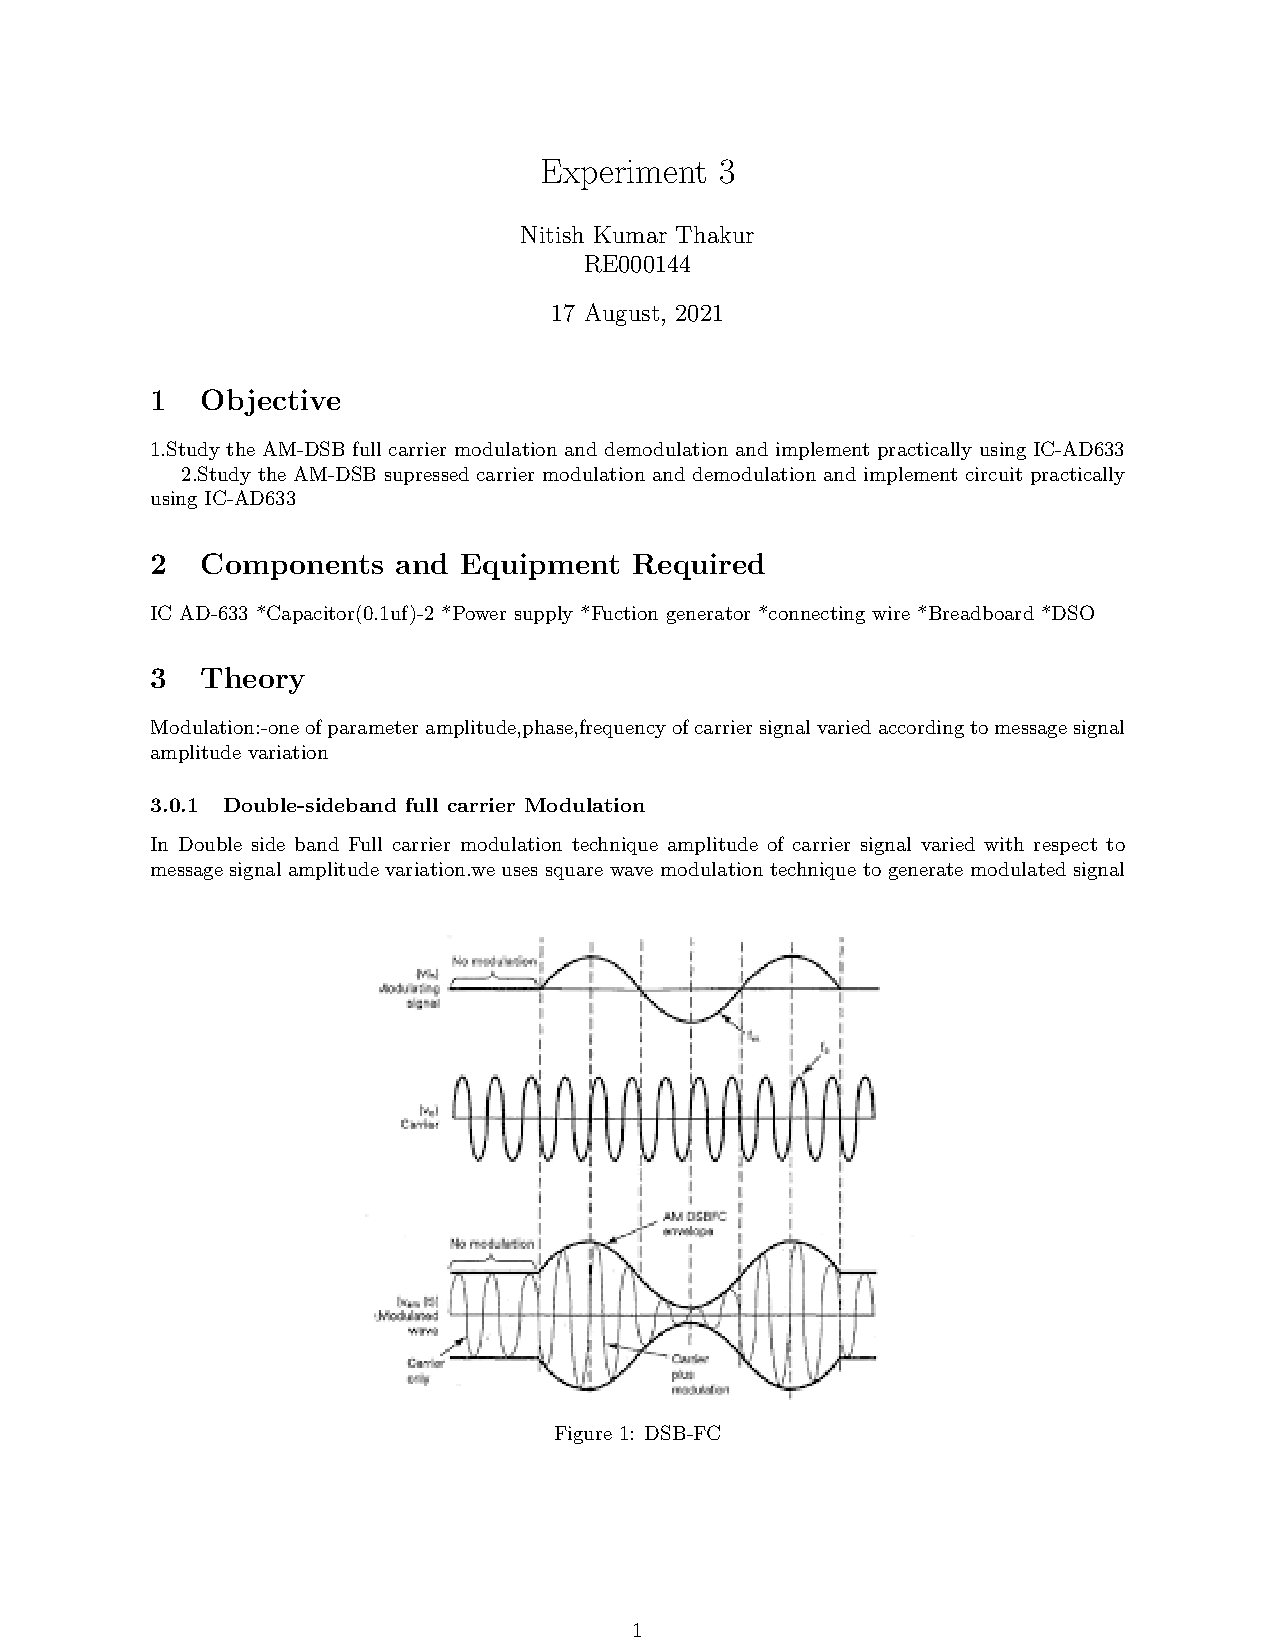
\includegraphics[width=\textwidth]{3.png}
    \caption{Supply voltage=0v}
    \label{fig:1}
  \end{subfigure}
  %
  \begin{subfigure}[b]{0.6\textwidth}
    \includegraphics[width=\textwidth]{4.png}
    \caption{Output waveform}
    \label{fig:2}
  \end{subfigure}
\end{figure}


\begin{figure}[ht]
  \begin{subfigure}[b]{0.6\textwidth}
    \includegraphics[width=\textwidth]{5.png}
    \caption{Supply voltage=1.1v}
    \label{fig:1}
  \end{subfigure}
  %
  \begin{subfigure}[b]{0.6\textwidth}
    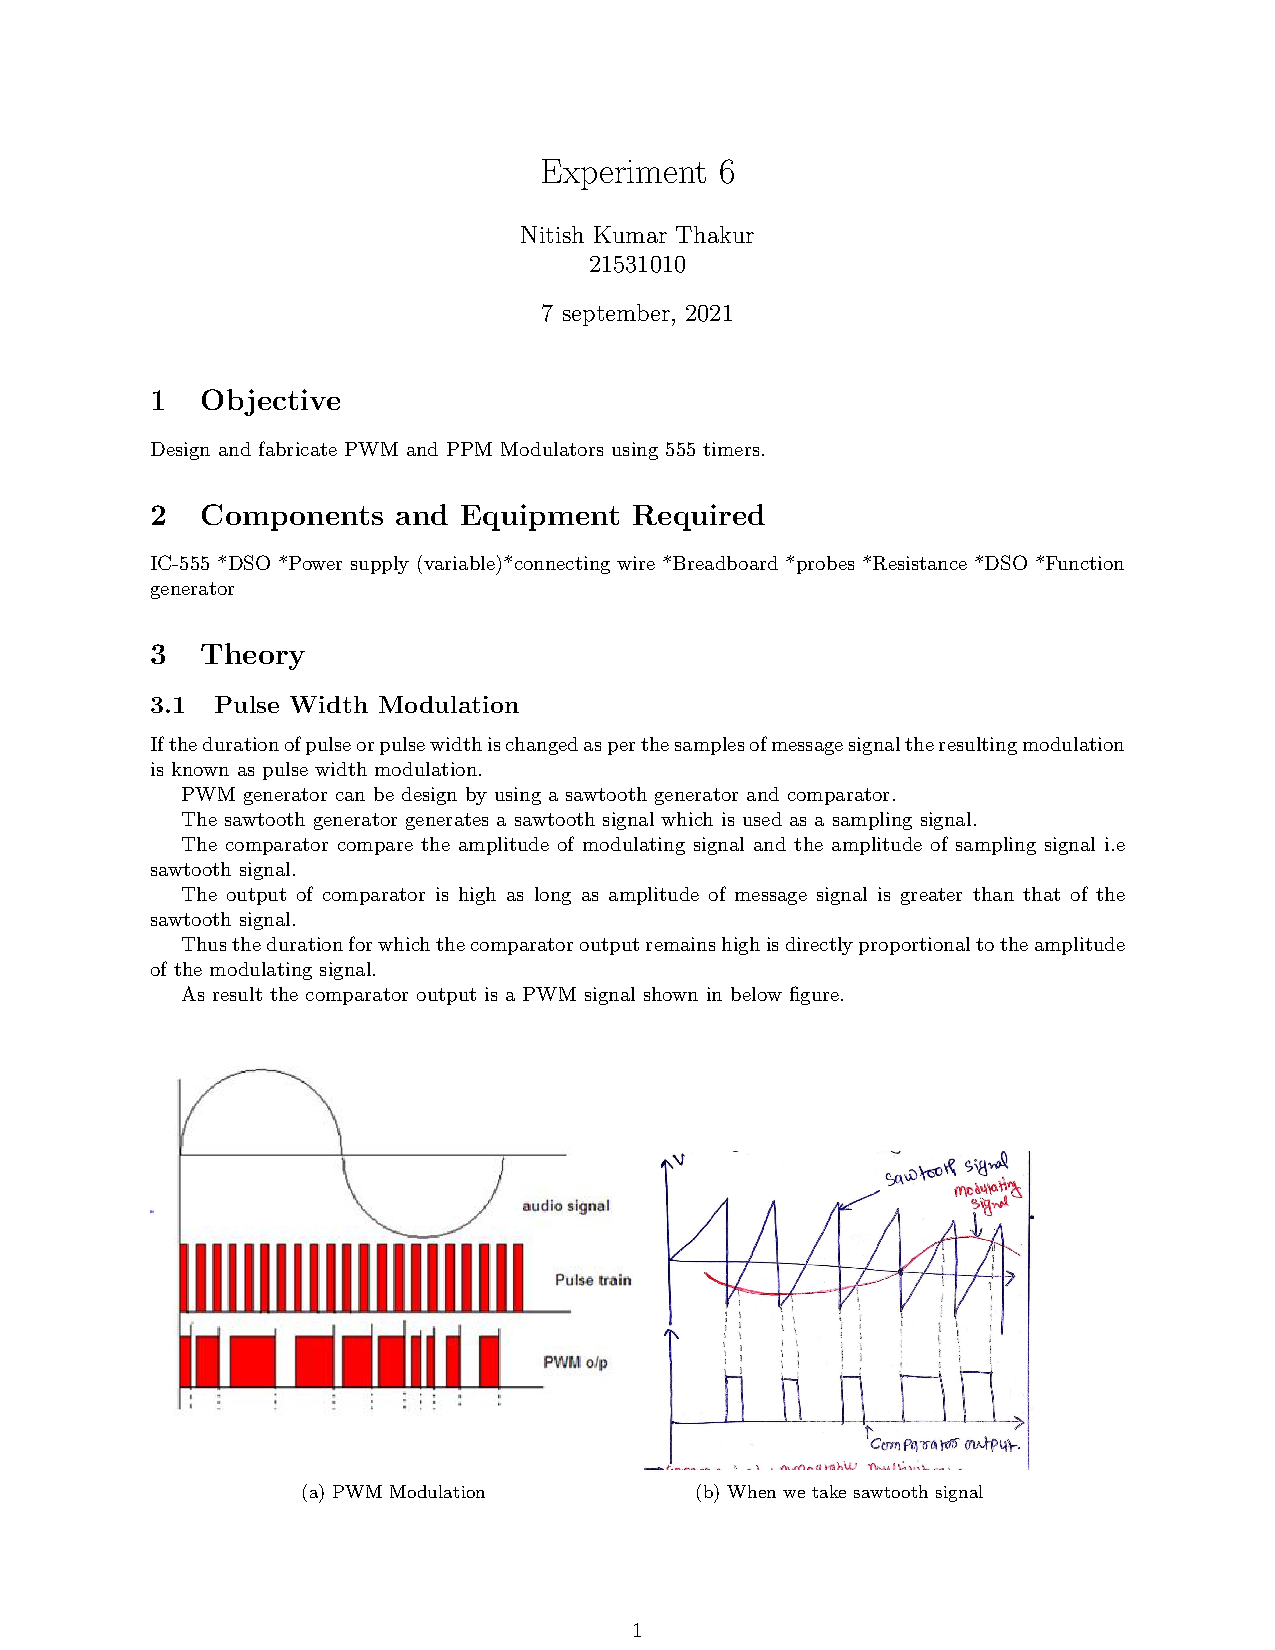
\includegraphics[width=\textwidth]{6.png}
    \caption{Output waveform}
    \label{fig:2}
  \end{subfigure}
\end{figure}


\begin{figure}[ht]
  \begin{subfigure}[b]{0.6\textwidth}
    \includegraphics[width=\textwidth]{9.png}
    \caption{Supply voltage=1.8v}
    \label{fig:1}
  \end{subfigure}
  %
  \begin{subfigure}[b]{0.6\textwidth}
    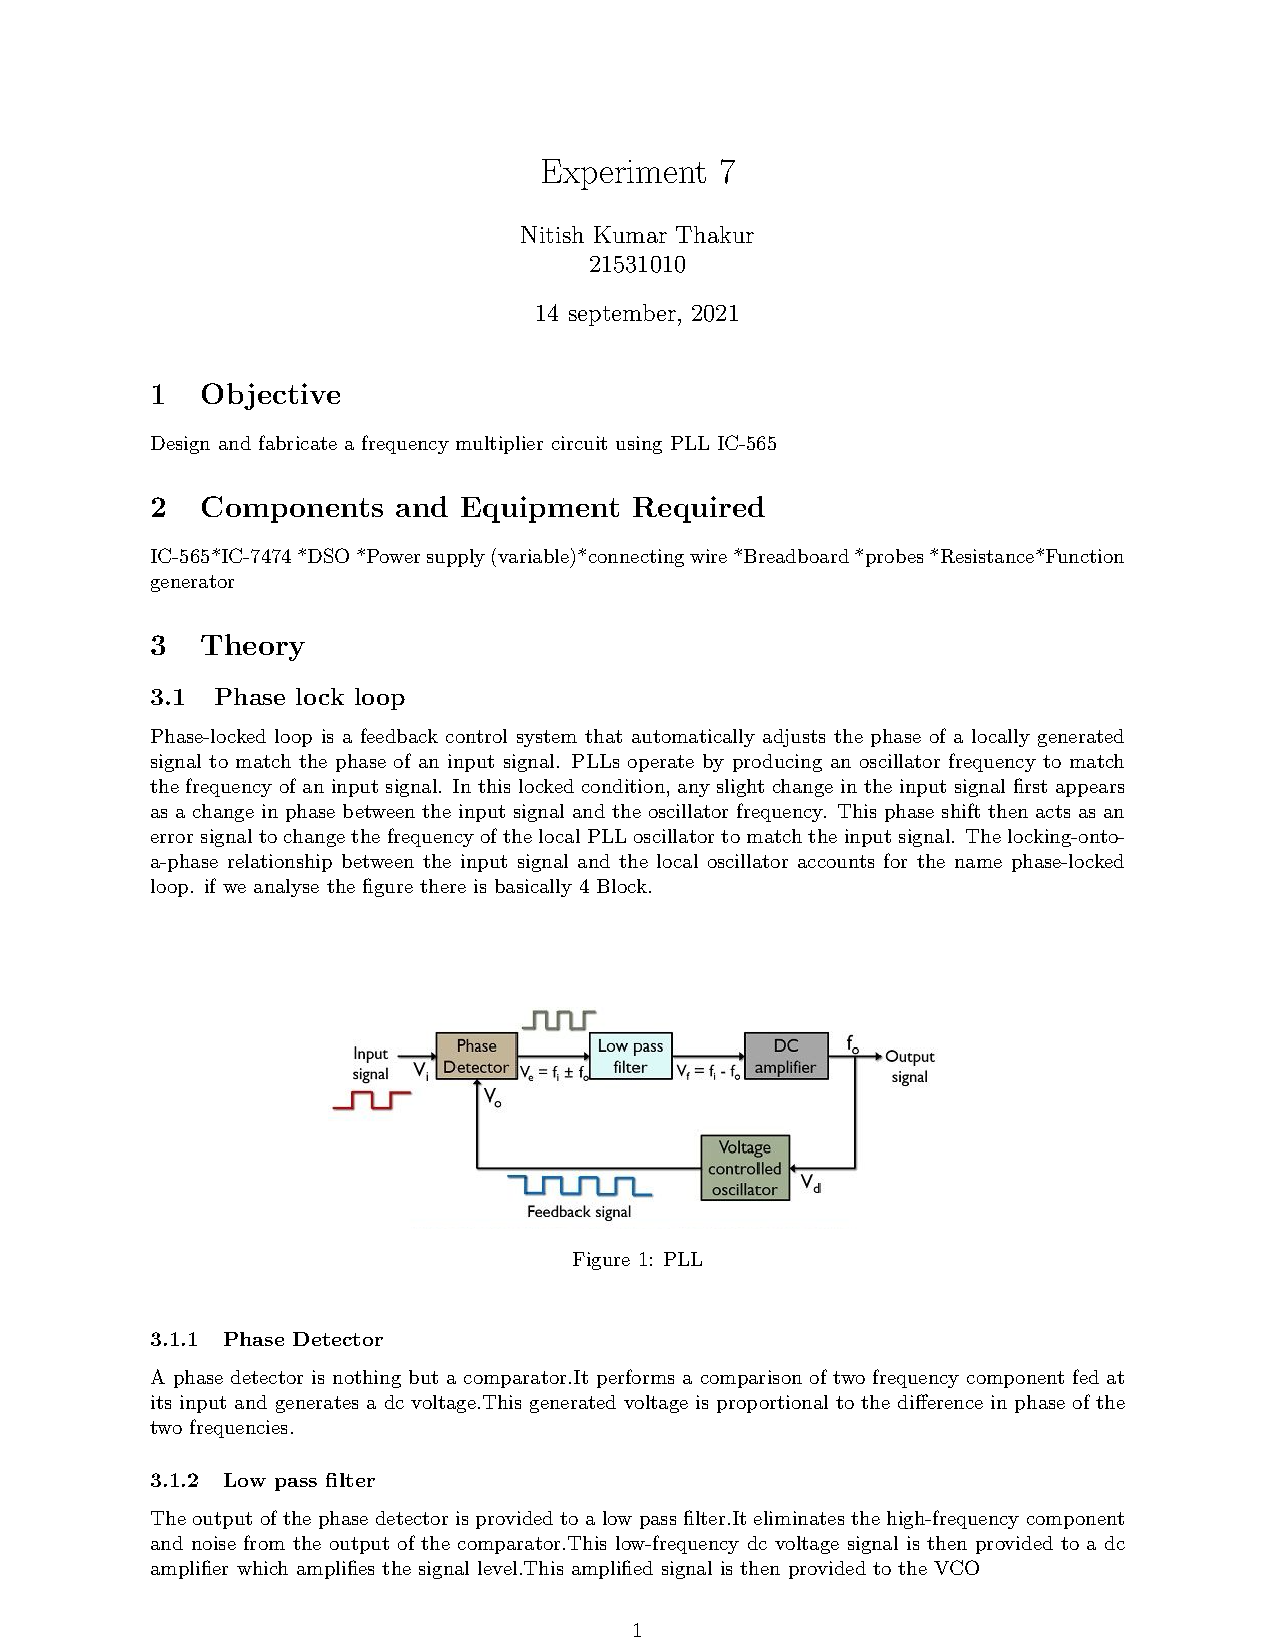
\includegraphics[width=\textwidth]{7.png}
    \caption{Output waveform}
    \label{fig:2}
  \end{subfigure}
\end{figure}

so we plot this varying frequency with respect to supply voltage and we observe that when supply voltage increases then frequency decreases.But in theoretically we studied that frequency is direct function of voltage but here when we increases the voltage, frequency is decreases. how this possible?Because when we connected the probe of power supply we connect in negative way that means we increases voltage but that's increases in Negative direction that means overall decreases so here voltage decreases.

\begin{figure*}[h]
	\centering
	\includegraphics[width=0.7\linewidth]{8.png}
	\caption{Supply voltage vs Frequency }
	\label{FD}
\end{figure*}

\subsection{FM modulation}
Pin-4,5 connected throught 10kohm resistor to 10 volt DC\par
Pin-6 connected to 10v DC\par

pin-9 connected to 10v through 10kohm resistor and also give square wave at pin-9\par
pin-10 connected throught 3.3nf capacitor to -10 volt DC\par
pin-11 connected directly -10v dc\par
pin-12 connected throught 82kohm resistor to -10 volt DC\par
pin-7,8 we supply sin wave (3 Vp-p,fm=820 Hz)\par
PIN-2 output taken\par  and observe that frequency is decreases or increases.when amplitude changes of sin wave.and we see when amplitude decreases then frequency decreases and when amplitude increases then frequency increases.

\begin{figure}[ht]
  \begin{subfigure}[b]{0.5\textwidth}
    \includegraphics[width=\textwidth]{10.png}
    \caption{Carrier signal}
    \label{fig:1}
  \end{subfigure}
  %
  \begin{subfigure}[b]{0.5\textwidth}
    \includegraphics[width=\textwidth]{11.png}
    \caption{Message signal}
    \label{fig:2}
  \end{subfigure}
\end{figure}
so Modulated signal is 

\begin{figure*}[h]
	\centering
	\includegraphics[width=0.5\linewidth]{12.png}
	\caption{Modulated signal}
	\label{FD}
\end{figure*}








\section{Conclusion/Sources of error}
 In this Experiment we study about Characteristic of VCO using IC-8038.and there is minor difference between Theoretical graph and practical graph.because we taken negative voltage.\par also if we observe the graph not exactlly linear beacause 
 and if we observe the DSO screen Frequency is varying when amplitude of message signal is varying(Frequency Modulation) this same thing we study Theoretically.
 
 
\end{document}
